%-----------------------------------------------------
% Chapter: Background 
%-----------------------------------------------------
\chapter{Background}
\label{chap:background}
This chapter provides an introduction to the theory and previous work within the areas of word embeddings, neural language models and text classification. 

\section{Word Embeddings}
Word embeddings are vectors of predefined size which aim to encode a distributional numerical representation of word features. Previous techniques for creating such representations can be categorised into two categories: matrix factorization methods and shallow window-based methods.
\subsection{Previous Methods}
\subsubsection{Global Matrix Factorization Methods}
Global matrix factorization methods such as Latent Semantic Analysis (LSA) use low rank approximations to decompose large matrices containing corpus statistics. Typically, these matrices take the form of a term-document matrix, which captures the frequencies of terms across a collection of documents, or a term-term matrix, which store co-occurrence counts of terms. Matrix factorisation methods such as LSA allow for fast training and perform well on word similarity tasks by leveraging word occurrence statistics however they suffer from the disproportionate importance given to large word counts.

\begin{figure}[h]
	\includegraphics[width=12cm, height=6cm]{./figures/fig12}
	\centering
	\caption[Matrix factorization of word-word co-occurence matrix]{Matrix factorization of a word-word co-occurrence matrix which approximates the co-occurrence matrix as the matrix multiplication of two word vectors with dimension \(D\). }
	\label{fig:fig12}
\end{figure}
\subsubsection{Shallow Window-Based Methods}
Shallow window-based methods provide an alternative approach to learning word representations by sliding a fixed window over the contents of a corpus and learning to predict either the surroundings of a given word (skip-gram model) or predict a word given its surroundings (continuous bag of words (CBOW)). In the case of shallow window-based methods, they are good at capturing more complex patterns and do well in the word analogy task, however they fail to leverage global statistical information such as those used in global matrix factorization methods.

\noindent
\newline
\begin{figure}[h]
	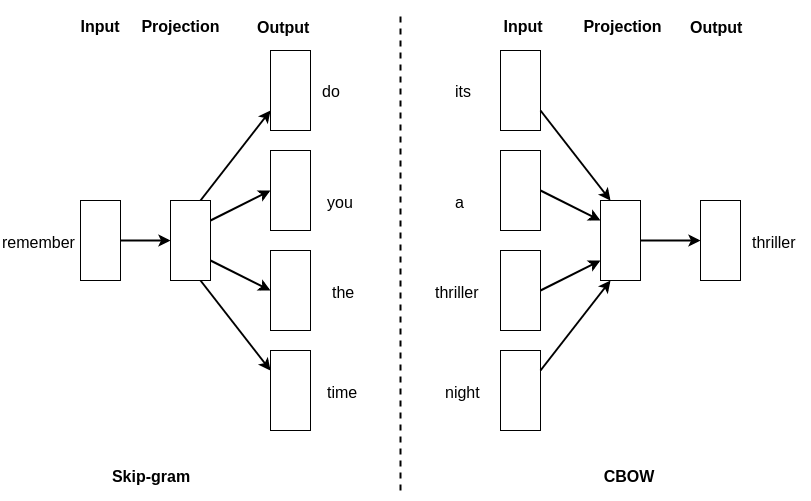
\includegraphics[width=12cm, height=8cm]{./figures/fig13}
	\centering
	\caption[Skip-gram and CBOW models]{Skip-gram models attempt to predict the proceeding and successive words of a given target word, whilst CBOW models attempt to predict a target word given its surrounding words}
	\label{fig:fig13}
\end{figure}
\subsection{GloVe}
Global Vectors for Word Representation (GloVe), is an unsupervised word embedding algorithm, introduced by \cite{Pennington2014}, which marries the benefits of both global matrix factorisation and shallow window-based methods. Presented as a log-bilinear regression model, GloVe makes use of global word co-occurrence statistics from a corpus. Specifically, given a  corpus, which has vocabulary size \(N\), a word-word co-occurrence matrix \(X\), with \(N\)x\(N\) dimensions, is computed with \(X_{ij}\) being a measure of the number of times words \(i\) and \(j\) co-occur within a given context window, which in GloVe is a inverse distance function, giving closer words higher counts. For example applying a right context window of size 3 over the sentence,

\begin{center}
	I'm looking at the man in the mirror
\end{center}

\noindent
and assuming the focal word was "man", the counts for its context words in the window would be computed as follows,

\begin{center}
	in: 1, \space
	the: \(\dfrac{1}{2}\), \space
	mirror: \(\dfrac{1}{3} \)
\end{center}

\noindent 
\newline
\newline
As detailed in the paper, GloVe outperformed previous methods such as word2vec in word analogy, word similarity and named entity recognition tasks, and as seen in \autoref{fig:fig16} is able to capture linguistic substructures.

\begin{figure}[h]
	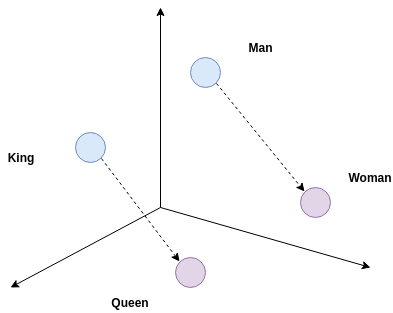
\includegraphics[width=8cm, height=6cm]{./figures/fig16}
	\centering
	\caption[Word Embedding Visualisation]{Example of the male-female relationship encoded in the word embedding space.}
	\label{fig:fig16}
\end{figure}

\noindent
Conceptually, GloVe is based on the idea that ratios of probabilities of words co-occurring with respect to another word, can encode more meaning than using the raw probabilities of the words co-occurring itself.

\noindent
\newline
This concept is formalised in the following equation, where the dot product of focal and context word vectors, \(w\) and \(\tilde{w}\) and their associated biases, \(b_{i} \) and \(\tilde{b}_{j}\), is approximately equal to the logarithm of the number of times the words co-occurred, \(\log{X_{ij}}\).

\begin{equation}
w_{i}^{T} \tilde{w_{j}} + b_{i} + \tilde{b}_{j} \approx \log{X_{ij}}^{2}
\end{equation}

\noindent
\newline
GloVe also utilises a weighting function \(f\) to decrease noise caused by rare word co-occurrences. The following weighting function is used in the GloVe model.

\begin{equation}
	f(x) =
	\begin{cases}
	(x/x_{max})^{\alpha}, & \text{if  \(x <\) } x_{max} \\
	1, & \text{otherwise}
	\end{cases}
\end{equation}

\noindent
\newline
Typically values of 0.75 and 100 are used for both \( \alpha \) and \(x_{max}\) respectively. Combining equations 4.1 and 4.2, the GloVe model is defined as a weighted least squares regression problem.
\begin{equation}
	J = \sum_{i, j=1}^{N} f(X_{ij}) (w_{i}^{T} \tilde{w_{j}} + b_{i} + \tilde{b}_{j} - \log{X_{ij}})^{2}
\end{equation}

\noindent
\newline
Training of GloVe utilises the AdaGrad optimiser (\cite{Duchi2011}) to perform stochastic gradient descent, which is an iterative method of optimising an objective function using small random samples of training data, in order to minimise the objective function above.

\noindent
\newline
\newline
\subsection{CoVeR}
Covariates such as author demographics, time and location often accompany documents within a corpus. A trivial approach to obtaining covariate specific word embeddings involves applying GloVe to each subset of corpus documents relating to a particular covariate. Unfortunately, utilising GloVe this way has certain drawbacks. Firstly, GloVe must be applied and optimised to each subset of corpus data, which, depending on the number of covariates, is computationally expensive. Also as a direct result of dividing the original corpus, global co-occurrence counts are now split across covariates. Consequently, global statistics are now not shared between embeddings, which may cause sub-optimal word representations, particularly when subsets of corpus data contain minimal amounts of co-occurrences for GloVe to train on. 

\noindent
\newline
Another issue with applying GloVe in this manner is interpretability. Apart from visual interpretation through dimensionality reduction and clustering as shown in Figure..., traditionally, interpreting the meaning of word vector dimensions has been challenging because of their random initialisation and due to the fact that dimensions are constructed relative to the order in which co-occurrence statistics are processed during training. As a result of this, applying GloVe this way makes it more challenging to relate the separate covariate word embeddings back together.


\noindent
\newline
Learning Covariate-Specific Vector Representations with Tensor Decompositions (CoVeR), proposed by \cite{Tian2018}, provides an alternative to the conditional GloVe method which offers a framework to making learned embeddings more interpretable and the learning process more data efficient. Being an extension of GloVe, CoVer extends Glove's matrix decomposition of a co-occurrence matrix \(X_{ij}\) to a tensor decomposition of a co-occurrence tensor \(X_{ijk}\) , involving the joint learning of word embeddings \(w\) and \(\tilde{w}\), a set of \(k\) covariate specific diagonal transformation matrices \(c\), which represent the effect of a particular covariate on the base embeddings learned and associated biases  \(b_{ik} \) and \(\tilde{b}_{jk}\) for words \(w_{i}\) and \(\tilde{w}_{j}\) in covariate \(k\) . Using the same weighting function as the GloVe method, the CoVeR model is presented below

\begin{equation}
J = \sum_{i, j=1}^{N} \sum_{k=1}^{M} f(X_{ijk}) ((c_{k} \odot w_{i})^{T} (c_{k} \odot \tilde{w}) + b_{ik} + \tilde{b}_{jk} - \log{X_{ijk}})^{2}
\end{equation}

\noindent
\newline
The introduction of covariate specific weight matrices into the objective function allows the authors to create covariate specific word embeddings by multiplying the base embeddings \(w\) and \(\tilde{w}\) by the covariate diagonal transformation matrix \(c_{k}\). This approach overcomes the limitations of data efficiency and interpretability in the conditional GloVe method by utilising global corpus statistics of all documents within a corpus, and providing a way to transform the base embeddings learnt into covariate specific embeddings through a covariate specific transformation matrix.

\noindent
\newline
The following sections introduce the two research areas which relate to the project goals, namely language modelling and text classification.


\section{Language Models}
Formal languages such as programming languages are fully specified with precise syntax and semantics which dictate the usage of all words reserved within the language. Contrarily, natural languages, because of their emerging nature, are unable to be formally specified even with the existence of grammatical rules and structures. Unfortunately, rule based systems for modelling language suffer from the endless possibilities of language usage outside of grammatical rules which are easily interpretable by humans. Moreover, the task of consistently updating rule based systems to accommodate such usage is unfavourable.  

\noindent
\newline
Language modelling (LM) is the task of estimating the probability distribution of various linguistic units such as characters, words and sentences. In recent years, the application of LM  has been essential to many NLP tasks such as Speech to Text and Text Summarization (\cite{Rush2015}). Language models can be classified into two categories, count-based and neural language models. 

\subsection{Count Based Models}
Count based models attempt to learn a probability distribution \(P(w_{1},...,w_{i}) \) over of a sequence of words \(w_{1},...,w_{i}\). An example of a count based model is the n-gram model.

\subsubsection{N-gram models}
An n-gram is a sequence of \(n\) words. Examples of two word sequences or bigrams include, \textit{"Annie are"} and \textit{"you okay"}, whilst examples of three word sequences or trigrams, include sequences of words such as \textit{"been hit by"} and \textit{"a smooth criminal"}. The n-gram model considers the past \(n-1\) words and uses Markov assumptions to approximate the probability of word sequences \(P(w_{1},...,w_{i}) \). This is formalised in the following equation

\begin{equation}
	P(w_{i} | w_{1},...,w_{i-1}) \approx P(w_{i} | w_{i-n+1},...,w_{i-1})
\end{equation}

\noindent
\newline
An inherent problem with the n-gram model is sparsity as some word sequences occur rarely or not at all, even in large text corpora. Using the standard n-gram model would yield too many zero probabilities. To mitigate this, techniques such as back-off (\cite{Katz1987}) and smoothing exist. Another disadvantage of the n-gram model is that they rely on exact matches, meaning they fail to recognise syntactically and semantically similar sentences such as \textit{"what about animals"} and \textit{"what about elephants"}. N-gram models also suffer from the curse of dimensionality due to increased vocabulary sizes. As a result, limited window sizes are used, causing longer dependencies between words not be captured.

\subsection{Neural Language Models}
To overcome issues faced by count based models, deep learning methods have been used to create neural language models by simultaneously learning word embeddings and the parameters needed to create a joint probability distribution between the word embeddings. \cite{Bengio2003} proposed a feed forward neural language model to help tackle the problem of data sparsity. Recent state of the art approaches such as \cite{Mikolov2010}, abstract language modelling as a form of sequential data prediction and have implored RNN's to help encode longer dependencies between sequences of words. The strength of these models comes from their ability to consider several preceding words and thus generalise well.

\noindent
\newline
An overview of generic neural network architectures as well as RNN's and LSTM's are given in the following sections.

\noindent
\newline
\newline
\subsubsection{Artificial Neural Networks}
In any neural network architecture, the elementary unit of computation is the artificial neuron which takes inspiration from biological neurons. The artificial neuron receives \(N\) inputs which are each weighted by \(N\) weights and summed together with a bias \(b\). The output \(y\) of a neuron is calculated by passing the weighted sum of the inputs into an activation function \(f\). 

\begin{equation}
	y = f\left( \sum_{i=1}^{N} x_{i}w_{i} + b\right)
\end{equation}

\noindent
\newline
Typical activation functions include the \textit{Sigmoid}, \textit{Tanh} and \textit{ReLu} functions. The equation above serves as the formula for the simplest king of network: a single layer network, also known as a perception. The process of stacking layers on top of each other leads to multi-layer neural networks. These types of networks are also known as feed-forward networks. The learnable parameters of these networks are the set of weights and biases for each layer. A feed-forward neural network is trained using gradient descent and its parameters are updated using the \textit{backpropagation} algorithm (\cite{Rumelhart1988}).

\begin{figure}[h]
	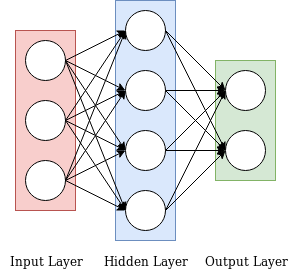
\includegraphics[width=8cm, height=8cm]{./figures/fig2}
	\centering
	\caption[Example fully connected feed-forward neural network]{Example of a fully connected feed-forward neural network with three input neurons, four neurons in the hidden layer and two output neurons.}
	\label{fig:fig2}
\end{figure}

\subsubsection{Recurrent Neural Network}
In a feed-forward neural network, data flow is unidirectional between layers; with data passing through a given neuron at most once. These types of networks perform well on both classification and regression tasks with the assumption that inputs are independent of each other. In tasks dealing with sequential data, feed-forward networks perform poorly. To model sequential data well, a neural network must be able to model the dependencies that exist between successive inputs. The recurrent neural network (RNN) is an attempt to satisfy this requirement by utilising past inputs to help predict future outputs.
\par
\noindent
\newline
In an RNN information is cycled within the network at least once.  An RNN receives a sequence of inputs \(x\) and updates its hidden state \(h_{t}\) by 

\begin{equation}
	h_{t}=
	\begin{cases}
	 0, & \text{t = 0} \\
	 \phi{(h_{t-1}, x_{t})}, & \text{otherwise}
	\end{cases}
\end{equation}

\noindent
where $\phi$ is a nonlinear function such as \textit{tanh} or \textit{ReLu}. The update for the hidden state is usually implemented as 

\begin{equation}
h_{t} = \phi{(Ux_{t} + Wh_{t-1})}
\end{equation}

\noindent
where W and U are weight matrices.

\par
\noindent
\newline
RNN's are trained using gradient descent and backpropagation through time (BBTT), which is identical to performing backpropagation on an \textit{"unrolled"} RNN (seen in figure \autoref{fig:fig3})

\begin{figure}[h]
	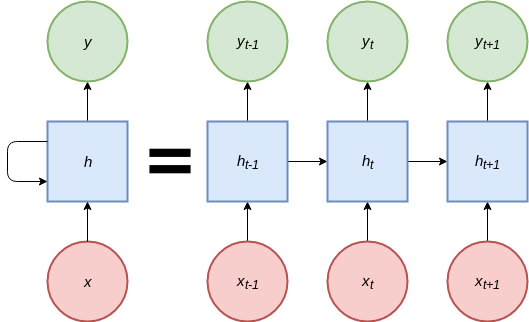
\includegraphics[width=10cm, height=6cm]{./figures/fig3}
	\centering
	\caption[Unrolled Recurrent Neural Network]{An \textit{unrolled} recurrent neural network can be seen as a feed-forward neural network with many hidden layers.}
	\label{fig:fig3}
\end{figure}

\par
\noindent
During BBTT, back propagation is performed on an unrolled recurrent architecture, causing gradients to back-propagate through numerous network layers. Unfortunately, this has a few major problems. Firstly, a single forward/backward pass through the network is computationally expensive due to the number of hidden layers of the unrolled network being linear to the number of time steps in a sequence. Secondly, this method suffers from the issue of vanishing or exploding gradients (\cite{Bengio1994}) where gradients can exponentially decay or grow as they propagate over time, which can prevent the network from learning entirely.
\subsubsection{Long Short-Term Memory}
Long Short-Term Memory (LSTM) (\cite{Hochreiter1997}) is a variant of the RNN which is capable of capturing longer dependencies between sequences of data without suffering from vanishing or exploding gradients. This is achieved through a feature known as gating; a mechanism which acts as a permissive or restrictive barrier to information flow. 

\noindent
\newline
The core component of the LSTM is the cell state which is able to propagate \textbf{relevant} information throughout the network. This is achieved within the memory cell through the forget, input and output gates. The forget gate controls how much existing memory should be forgotten, the input gate controls how much of the new cell state to keep, and the output gate controls how much of the cell state should be allowed into the next layer of the network. An example of an LSTM memory cell is seen in \autoref{fig:fig4}.

\begin{figure}[ht]
	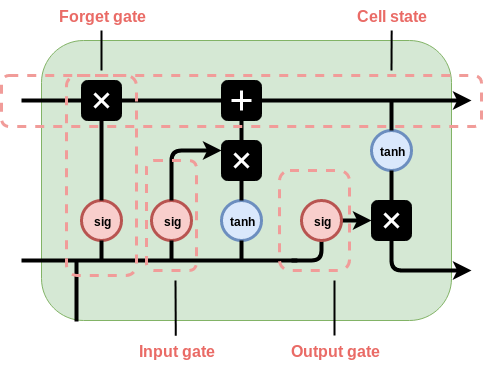
\includegraphics[width=10cm, height=8cm]{./figures/fig4}
	\centering
	\caption[LSTM Memory Cell]{LSTM memory cell, with forget, input and output gates}
	\label{fig:fig4}
\end{figure}

\subsection{Text Classification}
Text classification is the task of assigning pre-defined labels to text according to it's contents. Machine learning methods for text classification are preferred to rule based systems due to their ability to model regardless of domain. Text classification can be approached using supervised learning, where a model is trained with labelled training data, or unsupervised learning, where training data is clustered together to see if any natural grouping exists.

\noindent
\newline
Before a classifier can be trained, inputs must be transformed into numerical representations. A common method for creating such representations is the bag of words (BOW) approach which, given a vocabulary \(V\), with \(n\) words, creates a fixed size input vector of length \(n\) for document \(D\): representing word counts for each word in the vocabulary. For example, if we define the vocabulary \(V\) as being the set of words,

\begin{center}
\{"we", "are", "world", "children", "the"\}
\end{center}

\noindent
\newline 
and an input document \(D\) as being 

\begin{center}
\textit{"we are the world"} 
\end{center}

\noindent
\newline
the resulting representation for document \(D\) would be

\begin{center}
 [1, 1, 1, 0, 1] 
\end{center}


\noindent
\newline
Two popular machine learning methods for text classification include the naive Bayes classifier and the Support Vector Machine. They are briefly outlined in the following section.

\subsubsection{Naive Bayes}
Naive Bayes classifiers are a class of supervised probabilistic classifiers which have been used in text classification for tasks such as Spam Filtering (\cite{Sahami1998}). At their core, these types of classifiers rely on Bayes theorem which is shown below.

\begin{equation}
P(A|B) = \dfrac{P(B|A)P(A)}{P(B)}
\end{equation}

\noindent
The \textit{naivety} of these classifiers comes from the assumption of conditional independence between features. Specifically, given an input \(x\), with \(n\) features, and a target class y, naive Bayes classifiers use the following approximation to assign the probability of input \(x\) belonging to class \(y\).

\begin{equation}
P(x_{1},...,x_{n}|y) \approx \prod_{i=1}^{n}P(x_{i})
\end{equation}
\noindent
Given multiple classes, the classification of an input is given to the class with the maximum conditional probability as shown in the equation above. This is generalised in the formula below.

\begin{equation}
y = argmax_{y} P(y) \prod_{i=1}^{n}P(x_{i} | y)
\end{equation}

\subsubsection{Support Vector Machines}
Support Vector Machines (SVM) (\cite{Cortes1995}) have also been applied successfully to text classification problems (\cite{Joachims1998}). Unlike naive Bayes classifiers, SVM's are discriminative classifiers which aim to find a hyperplane in N-dimensional space which maximises the margin between data points of different classes. This is achieved through the use of random data points, namely \textit{"support vectors"}, which are data points closest to the hyperplane which help maximises the margin distance between classes. Maximising marginal distance between classes provides confidence to the classification of future data points.

\noindent
\newline 
\begin{figure}[ht]
	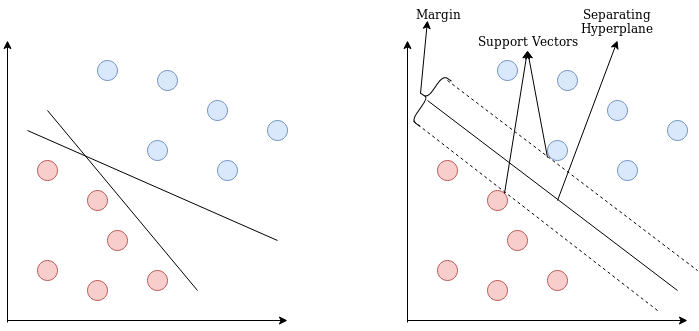
\includegraphics[width=12cm, height=5.5cm]{./figures/fig17}
	\centering
	\caption[Support Vector Machine]{Support Vector Machine - The left set of data points can be linearly separated by many lines, but the goal of the SVM on the right is to use the support vectors to maximise the margin between the two classes. The optimal separating hyperplane is in the middle of this maximised margin}
	\label{fig:fig17}
\end{figure}

\subsubsection{Deep Learning Methods}
Until recently, state of the art methods for text classification had long used linear predictors such as the SVM (with a linear kernel) and multinomial naive Bayes classifiers using feature representation techniques such as bag-of-words (\cite{Joachims1998} \cite{Lewis2004}). However, non-linear methods that are able to leverage dependencies between words ,such as recurrent neural networks, have provided better predictions (\cite{Dai2015a}) than previous bag-of-word approaches where features are assumed to be conditionally independent and unordered.